\documentclass[output=paper]{langsci/langscibook} 
\title{Daatsʼíin, a newly identified undocumented language of western Ethiopia: A preliminary examination} 
\author{%
 Colleen Ahland \affiliation{SIL International} 
}
% \chapterDOI{} %will be filled in at production


\abstract{
Daats’íin is a heretofore unknown language spoken in western Ethiopia near the border with the Republic of Sudan. The Daats’iin people live in both Ethiopia and the Republic of Sudan but only those in Ethiopia still speak the Daats’iin language. The speakers of Daats’íin may number around 1,000 but may be as few as 300-500. This paper provides the first-ever overview of basic aspects of Daatsʼíin phonology, morphology and syntax. The overview documents that Daatsʼiin is structurally similar to the nearby Gumuz languages (of possible Nilo-Saharan affiliation) in many respects, including vocabulary, bound pronominals with a distinct tone for S versus A arguments, and incorporated nouns. However, there are a few differences, mainly in structure and certain tense-aspect categories of the verb word. 
}
\shorttitlerunninghead{Daatsʼíin, a newly identified undocumented language of western Ethiopia}
\maketitle
\begin{document}

%Keywords: Daatsʼíin, Gumuz, language isolates, endangered languages, Nilo-Saharan, Ethiopian languages

\section{Introduction}\label{sec:ahlandc:1}

Daatsʼíin is the self-name of a people group living in western Ethiopia and the southern part of the Republic of Sudan. The Daatsʼíin in Sudan have lost their traditional language but those in Ethiopia still speak it. Up until 2013, the language and people group were unknown to researchers and not included in the Ethiopian Census. I traveled to the area in 2014 in order to investigate the language and confirmed that Daatsʼíin (ISO dtn) is distinct from but closely related to Gumuz (ISO guk). I estimate that the Daatsʼíin likely number less than 1000 and that their language may be in danger of dying due to their population size and the heavy influence of Arabic and Amharic in the area.

Following is a first ever description and analysis of the Daatsʼíin language based on a word list of 400+ words,\footnote{These are the first 300 words of the SIL Comparative African Wordlist \citep{SniderRoberts2006} plus words gleaned from texts which matched other items on the wordlist. Individual words were also collected for the Leipzig-Jakarta wordlist of the “least borrowable” words \citep{HaspelmathTadmor2009}. See Appendix.} five translated and annotated texts, and forty-four hours of targeted elicitation gathered in Ethiopia during a May-June 2014 field trip. The texts were gathered from Daatsʼíin adult native speakers of various ages, both male and female from the village of Mahadid, Qwara wereda, Amhara Region. The word list and elicitation sessions were conducted with a male native speaker in his late 20’s from Mahadid village. In \sectref{sec:ahlandc:2} I present the locations of villages where Daatsʼíin is known to be spoken and give an overview of the similarities and differences between Daatsʼíin and Gumuz. In \sectref{sec:ahlandc:3}, I present a brief phonological analysis. In \sectref{sec:ahlandc:4} I present the verbal morphology, in \sectref{sec:ahlandc:5} describe the reciprocal construction, and in \sectref{sec:ahlandc:6} various voice constructions. I then move on to noun morphology in \sectref{sec:ahlandc:7} and noun modification in \sectref{sec:ahlandc:8}. In \sectref{sec:ahlandc:9} I present demonstratives and in \sectref{sec:ahlandc:10} describe prepositions and spatial relations. Lastly, in \sectref{sec:ahlandc:11} I cover syntax. I end the grammatical description with a brief conclusion in \sectref{sec:ahlandc:12}.

\section{Background}\label{sec:ahlandc:2}

\subsection{Location}\label{sec:ahlandc:2.1}

In Ethiopia, the Daats’i\'{ }in live in small villages within Mahadid K’ebele, northwest of Gelegu (formerly “Tewodros Ketema”), the capital of Qwara wereda, Amhara Region, near the edge of Alatish National Park. The Daats'íin also live in villages of Inashemsh (Emshemis?) K’ebele near Omidla in Guba wereda, Benishangul-Gumuz Region (\figref{fig:ahlandc:1}).\footnote{The location of Mahadid village is based on a GPS reading: 12º17'56''N, 35º45'48''E.  The location of Inashemsh is approximate, based on a description given by a Daats’íin language consultant.} In Sudan, ethnic Daats’íin live in the villages of Ba’asinda and Gotihayaf.\footnote{The village names (other than Mahadid) were given to me by a Daatsʼíin language consultant; I have not visited these locations to confirm whether ethnic Daatsʼíin live there. }

 
\begin{figure}
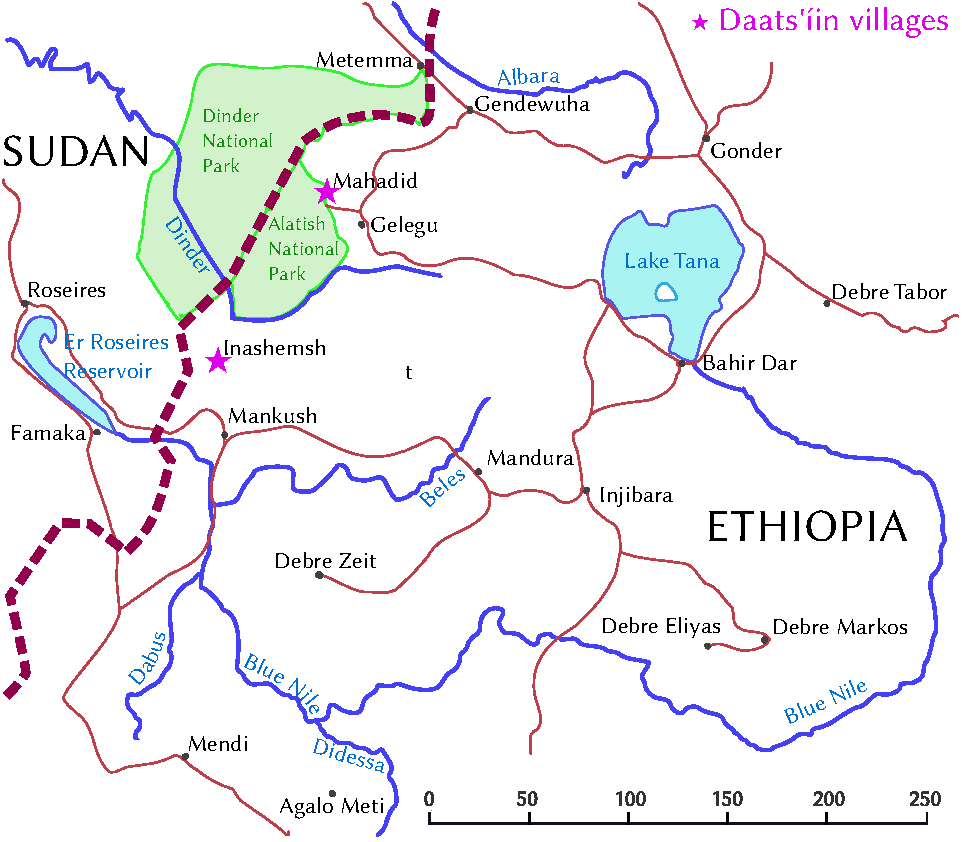
\includegraphics[width=\textwidth]{figures/AhlandCDaatsiin.pdf}
\caption{Daats’íin villages in Ethiopia (based on a map by SIL)}
\label{fig:ahlandc:1}
\todo[inline]{remove lines left and on top; put towns on road intersections}
\end{figure}

\subsection{Relationship to Gumuz}\label{sec:ahlandc:2.2}

Daatsʼíin and the Gumuz languages are very similar and would appear to be dialects of the same language if one merely inspected a wordlist (see Appendix). However, there exist quite a few differences grammatically, many of which explain the reported lack of mutual intelligibility between the languages.\footnote{I witnessed Gumuz and Daatsʼíin neighbors using Arabic or Amharic to communicate with one another. In some cases, the Daatsʼíin have learned the Gumuz language. However, I know of no instances where a Gumuz has learned to speak Datsʼíin. Both groups claim to not understand the other’s language unless they have learned it.}

While verb roots in Daatsʼíin and Gumuz are mostly cognate, the verbal morphology is very different in some respects. For both Daatsʼíin and the Gumuz languages, verbs are often polysynthetic \REF{ex:ahlandc:1}-\REF{ex:ahlandc:2}.\footnote{All language examples are written phonemically including the predictable epenthetic /a/ (in both Daatsʼíin and Gumuz), which also carries tone. Examples not written phonemically appear in phonetic brackets [ ].} Much verbal morphology in these languages is presumed cognate, but certain cognate morphemes appear in different orders on the verb, such as the directional morpheme /-é/\footnote{When the directional /-e\'{ }/ \textsc{twrd} occurs on a non-motion verb, it indicates that the speaker went to a location and came back (see also \citealt{Ahland2012}).} \REF{ex:ahlandc:1} and incorporated prepositions like the Dative (\textsc{dat}) \REF{ex:ahlandc:2}.

\ea\label{ex:ahlandc:1}
\ea\label{ex:ahlandc:1a}  
Daatsʼíin  \\
\gll
ákwá    má-ba-ŋ-gáŋ-gám-ákwa-ts-é\\
\textsc{1pl.incl.pro}   \textsc{imp-1pl.incl.imp-vr-redup}-know-\textsc{1pl.incl-body-twrd}\\
\glt ‘We see each other over there.’ \\

\ex\label{ex:ahlandc:1b}  
Southern Gumuz \\
\gll
 ákwa    kâm-a-gam-ágw-é-ts \\
  \textsc{1pl.incl.pro}   \textsc{fut-recp-}know-\textsc{1pl.incl-twrd-body}\\ 
\glt ‘We will see each other over there.’
\z
\z

\ea\label{ex:ahlandc:2}
\ea\label{ex:ahlandc:2a} 
Daatsʼíin\\
\gll
áljá                 ká=járʔám        k-ila-ca-ká  \\
\textsc{1pl.excl.pro} \textsc{dat}=\textsc{3pl.pro}   \textsc{aff-1pl.excl.tr-}give-\textsc{dat} \\
\glt ‘We gave to him.’ \\

\ex\label{ex:ahlandc:2b}  
Southern Gumuz \\
\gll
  áíla                 b-íl-ká-cá-gá  ká=áŋ \\
\textsc{1pl.excl.pro} \textsc{aff-1pl.excl.tr-dat-}give-\textsc{nfut}  \textsc{dat=3sg.pro} \\
\glt ‘We gave to him.’
\z
\z

Certain  verbal morphemes only exist in Gumuz and not Daatsʼíin – e.g.\ the uncertainty prefix, perfect aspect suffix, nonfuture (\textsc{nfut)} suffix \REF{ex:ahlandc:2b} \citep{Ahland2012} – and  vice versa, i.e.\ a unique 1\textsc{pl} inclusive prefix \textit{ba- }that co-occurs with the bound pronominal is found only in Daatsʼíin \REF{ex:ahlandc:1a}. In addition, some verbal morphemes in Daatsʼíin and Gumuz that perform the same function are non-cognate, e.g.\ the remote past tense (/é-/ in Southern Gumuz and /-b/ in Daatsʼíin) (see \sectref{sec:ahlandc:4.4}, the affirmative prefix (/k-/ in Daatsʼíin as in \REF{ex:ahlandc:2a}, but /b-/ in Southern Gumuz as in \REF{ex:ahlandc:2b}, and /d-/ in Northern Gumuz), and the relativizer (\sectref{sec:ahlandc:10}). Also, the verbal plural (pluractional) is the result of a morphological process in Daatsʼíin (\sectref{sec:ahlandc:4.7}), but is expressed as the prefix /N-/ in the Gumuz languages.

Moreover, the Gumuz languages utilize two verbal templates based on tense: future \REF{ex:ahlandc:1b} versus nonfuture \REF{ex:ahlandc:2b}; while the two Daatsʼíin verbal templates are based on aspect: imperfective \REF{ex:ahlandc:1a} versus perfective \REF{ex:ahlandc:2a}.This would no doubt result in miscommunication as the ‘future’ form in Southern Gumuz (used mainly to express future time events) is similar to and presumed cognate with the ‘imperfective’ form in Daatsʼíin (which can be used to express a past event). The future template in Northern Gumuz utilizes a non-cognate future tense morpheme.\footnote{Northern Gumuz has a less commonly used ‘future’ form which I presume is cognate to that of Southern Gumuz and Daatsʼíin. I tentatively label this form \textit{immediate future} \citep[233]{Ahland2012}.}


Lastly, while verbs are often inflected with bound pronominals in Daatsʼíin, this inflection is not required. One can simply use the free pronoun without inflecting the verb for person. This is not true for either Northern or Southern Gumuz; verbs must be inflected for person.

Therefore, while Daatsʼíin and the Gumuz languages are very similar, there are several reasons to categorize these as distinct languages: lack of mutual intelligibility, distinct ethnolinguistic identity, and differing grammatical structures. These languages (Daatsʼíin, Northen Gumuz, Southern Gumuz) form their own subgroup within Nilo-Saharan or possibly stand as an independent isolate family, as proposed for Gumuz by \citet{Dimmendaal2011}. In what follows the discussion will primarily focus on Daatsʼíin as a hitherto undocumented language, but occasional comparisons with Gumuz will be noted.


\section{Phonology}\label{sec:ahlandc:3}


The Daats’íin phonological inventory includes 33 consonants (\tabref{tab:ahlandc:1}), and 5 vowels (\tabref{tab:ahlandc:2}) with some contrast in vowel length. Daats’íin has two tones: H and L. In this paper, H tone is indicated with an acute accent mark while L tone is unmarked. Downstepped H tones are marked with \textsf{ꜜ }before the affected tone.


\subsection{Consonants}\label{sec:ahlandc:3.1}

Daats’íin consonants span six places of articulation. Phonetically labialized consonants occur, but unlike for Gumuz these are not phonemic. Also noteworthy is the existence of a phonetic pharyngeal fricative. However, I do not consider it phonemic as the distribution is limited and predictable to some extent. Lastly, the language has both ejective and implosive stops.  

\begin{table}
\begin{tabularx}{\textwidth}{lXXXXXXXXXXXX} \lsptoprule & \multicolumn{2}{X}{Labial} & \multicolumn{2}{X}{Alveolar} & \multicolumn{2}{X}{Alveo-Palatal} & \multicolumn{2}{X}{Palatal} & \multicolumn{2}{X}{Velar} & \multicolumn{2}{X}{Glottal} \\
\midrule
Stop & p   &     b & t    &      d &  &  & c     &    ɟ & k    &    g & ʔ& \\
{\ \ \ } glottalized & pʼ    &   ɓ & tʼ     &    ɗ & &  & cʼ & & kʼ & & & \\
Affricate & & & ts & & tʃ & & &  &  & & & \\
{\ \ \ } glottalized & & & tsʼ & & tʃʼ & & & & & & & \\
Fricative & f    &    (v) & s     &     z &  & & ʃ    &     (ʒ) & &  & h & \\
Nasal & m & & n & & &  & &  & ŋ & & & \\
Approximant & & & & & & & & & & & & \\
{\ \ \ } lateral & &  & & l & &  & &  & &  & & \\
{\ \ \ } flap/trill & &  & & r & & & & & & & & \\
Semi-vowel & w & & &  &  & & j & & &  & & \\
\lspbottomrule
\end{tabularx}
\caption{Daats’íin consonant phonemes}
\label{tab:ahlandc:1}
\end{table}

The palatal stop allophones [c, c’, ɟ] of /c/, /cʼ/ and /ɟ/ are in free variation with palatalized velar stop allophones [kʲ , kʼʲ, gʲ], respectively. This is similar to Gumuz palatal stops. However, in most Gumuz dialects, the palatal stop pronunciation appears to be preferred over the palatalized velar stop pronunciation; in Daatsʼíin, the palatalized stop pronunciation seems to be preferred. 

Marginal phonemes are in parentheses in \tabref{tab:ahlandc:1}. The consonants /v/ and /ʒ/ have highly limited distributions. The consonant /v/ is only found in one word thus far /vako/ ‘bone’, but exhibits contrast with similar segments in analogous environments. 

\ea
\begin{tabular}{llllll}
v & & f & & b & \\
/vako/   &  ‘bone’  &   /fago/  &   ‘be drunk’  & /bakaʔííba/ & ‘s/he who had’  \\           
& & /kʼ\'{o}faku/ &  ‘navel’ & & \\
\end{tabular}
\z

Likewise, /ʒ/ is only found in the root /ʒiɟ/ ‘sleep’. However, there is clear contrast with /z/ before a short /i/. With further data, it may be proven that the /ʒ/ in ‘sleep’ is simply an allophone of /z/ when the following consonant is palatalized or is a palatal stop. As discussed above, palatalized stops (e.g.\ [gʲ]) and palatal stops (e.g.\ [ɟ]) are in free variation. 

\ea
\begin{tabular}{llll}
ʒ  & &   z & \\
/ʒiɟ/ &  ‘sleep’  &  /ázil-kʼo/ & ‘bend down, stoop‘\\
\end{tabular}
\z

The glottal stop /ʔ/ is realized as a voiced pharyngeal fricative [ʕ] following a sonorant and in the environment of the low vowel /a/, as in \REF{ex:ahlandc:3a}. If a non-low vowel follows the glottal stop, the latter is realized as a phonetic glottal stop regardless of whether a sonorant precedes \REF{ex:ahlandc:3b}. If no sonorant precedes, the glottal stop surfaces as a glottal stop [ʔ], regardless of the surrounding vowels \REF{ex:ahlandc:3c}.

\ea\label{ex:ahlandc:3}
\ea\label{ex:ahlandc:3a} [jarʕam] \textsc{3S pro} 
\ex\label{ex:ahlandc:3b} [jarʔii] ‘be black’
\ex\label{ex:ahlandc:3c} [baʔás] ‘three’
\z
\z


\subsection{Vowels}\label{sec:ahlandc:3.2}

The vowel inventory of Daats’\'iin (\tabref{tab:ahlandc:2}) could be argued to consist of five vowels but with length contrasts realized by a difference in vowel quality. This is most noticeable with the realization of short /a/ as [ə]. Vowel quality differences are less pronounced (perhaps non-existent) for the mid-vowels /e/ and /o/. Thus, there appears to be no length contrast for the mid-vowels. Contrast between the long [i] and short [ɨ] high front vowels is similar to typical ATR contrasts found in many other African languages: [i] vs. [ɪ].


\begin{table}
\begin{tikzpicture}[baseline=default, on grid=true, scale=.4]
\aeiou 
\end{tikzpicture}
 
\caption{Daatsʼíin vowel phonemes}
\label{tab:ahlandc:2}
\end{table}


The short round vowel /u/ is optionally realized as a labiovelar approximant followed by a high central vowel: [wɨ]. \tabref{tab:ahlandc:3} shows posited length contrasts for the high vowels in all environments and between long and short /a/ word-medially. There is no known contrast for long and short /a/ word-initially, and only few examples word-finally. The phonetic realization of what I analyze as length contrasts are given in brackets.


\begin{table}

\begin{tabularx}{\textwidth}{lXXXXXX}
\lsptoprule
& \multicolumn{3}{l}{Short Vowel} & \multicolumn{3}{l}{Long Vowel}\\
\midrule
\mdseries /i/ & \mdseries /i\'{ }l-kʼ\'{o}/ & \mdseries [ɨlkʼ\'{o}] & \mdseries ‘head’ & \mdseries /ííl/ & \mdseries [íl] & \mdseries ‘belly’\\
/u/ & /af\'{u}tʃʼa/ & \mdseries [afwɨtʃʼa] & \mdseries ‘blow’ & \mdseries /fu\'{ }\'{u}na/ & \mdseries [f\'{u}nna]\footnote{In this particular word, long /uu/ is realized as a short [u] followed by a lengthened nasal.} & \mdseries ‘smell’\\
/a/ & /ham/ & [həm] & {\mdseries ‘gall bladder’} & {\mdseries /aha\'{ }áma/} & [aháma] & {\mdseries ‘yawn’} \\
& /baʃok/ & [bəʃok] & \mdseries ‘porcupine’ & /mbaaʃia/ & [m̩baʃija] & ‘hide \\
& & & & & &  (v, tr.)’\\
\lspbottomrule
\end{tabularx}
\caption{Posited vowel length contrasts}
\label{tab:ahlandc:3}
\end{table}


While /o/ does not appear to have a contrast in length with short /o/ being realized as [wə], for example, the vowel often varies with labialization on a previous (back) consonant. 


\subsection{Tone}\label{sec:ahlandc:3.3}

Daats’íin has two tones, H and L, as represented in the near minimal pairs in \REF{ex:ahlandc:4} and \REF{ex:ahlandc:5}. Preliminary analysis suggests that Daatsʼíin also exhibits downstepped H tones. For example, the final L tone of the HL pattern on intransitive (S)\footnote{I use the notation S, A, and P in the vein of \citet{Comrie1989}: S is the single core argument in an intransitive subject function, A is the argument of a transitive clause that correlates most closely with the notion of \textit{Agent}, and P is the argument of a transitive clause that correlates most closely with the notion of \textit{Patient}.} bound pronominals (\tabref{tab:ahlandc:4} in \sectref{sec:ahlandc:4.2}) induces a downstepped H tone on a following H-initial morpheme (see \tabref{tab:ahlandc:5} in \sectref{sec:ahlandc:4.2}). 

\ea\label{ex:ahlandc:4}

\begin{tabular}{ll}
LL &   HH  \\
/giʃa/  &    /gíʃí/ \\
‘stone(s)’    &  ‘see’ \\
 \end{tabular}
\z

\ea\label{ex:ahlandc:5}

\begin{tabular}{ll}
LHL   &     LH \\
  /afága/   &  /fagá/ \\
  ‘urinate’  &  ‘grow (up)’ \\
\end{tabular}
\z 

\section{Verb morphology}\label{sec:ahlandc:4}

Daats’íin verbs are somewhat polysynthetic with up to eleven position classes (and possibly more). While both prefixes and suffixes are possible, verbs are more heavily suffixing. There exist two templates for Daats’íin verbs: one for perfective verbs (\figref{fig:ahlandc:2}) and one for imperfective verbs (\figref{fig:ahlandc:3}).

\begin{figure}
\begin{tabularx}{\textwidth}{XXXXXXXXXXp{2cm}}
\begin{turn}{33} Mood \end{turn} & \begin{turn}{33} Person (S/A) \end{turn} & \begin{turn}{33} Valence Decreaser \end{turn} & \begin{turn}{33} Main Verb Root \end{turn} & \begin{turn}{33} Greater Plural \end{turn} & \begin{turn}{33} Past \end{turn} & \begin{turn}{33} Middle Voice \end{turn} & \begin{turn}{33} Instrumental \& Dative \end{turn} & \begin{turn}{33} Person (object of preposition) \end{turn} & \begin{turn}{33} Incorporated Noun \end{turn} & \begin{turn}{33} Directional \end{turn} \\
\midrule
\multicolumn{1}{X}{{}-3} & \multicolumn{1}{X}{{}-2} & \multicolumn{1}{X}{{}-1} & \multicolumn{1}{X}{0} & \multicolumn{1}{X}{+1} & \multicolumn{1}{X}{+2} & \multicolumn{1}{X}{+3} & \multicolumn{1}{X}{+4} & \multicolumn{1}{X}{+5} & \multicolumn{1}{X}{+6} & +7\\
\end{tabularx}
\caption{Position class chart for Daatsʼíin perfective verbs}
\label{fig:ahlandc:2}
\end{figure}

\begin{figure}
\begin{tabularx}{\textwidth}{XXXXXXXXp{3cm}}
\begin{turn}{33} Imperfective \end{turn} & \begin{turn}{33} 1PL Inclusive \end{turn} & \begin{turn}{33} Main Verb Root \end{turn} & \begin{turn}{33} Past \end{turn} & \begin{turn}{33} Greater Plural \end{turn} & \begin{turn}{33} Person (S/A) \end{turn} & \begin{turn}{33} Incorporated preposition \end{turn} & \begin{turn}{33} Directional \end{turn} & \begin{turn}{33} Incorporated Noun \end{turn} \\ \midrule
\multicolumn{1}{X}{{}-2} & \multicolumn{1}{X}{{}-1} & \multicolumn{1}{X}{0} & \multicolumn{1}{X}{+1} & \multicolumn{1}{X}{+2} & \multicolumn{1}{X}{+3} & \multicolumn{1}{X}{+4} & \multicolumn{1}{X}{+5} & +6\\
\end{tabularx}
\caption{Position class chart for Daatsʼíin imperfective verbs}
\label{fig:ahlandc:3}
\end{figure}

One of the main differences between the two templates is the position of the S/A bound pronominal. For the perfective template, the S/A bound pronominal is a prefix to the verb root \REF{ex:ahlandc:6}. For the imperfective template, the pronominal is a suffix \REF{ex:ahlandc:7} save for the 1\textsuperscript{st} person plural inclusive, which is doubly marked in the imperfective with both a prefix and a suffix. 

\ea\label{ex:ahlandc:6}
\gll 
k-\textbf{íl}{}-dugwa \\
\textsc{aff}{}-\textbf{\textsc{1pl.incl.intr}}{}-run \\
\glt
‘We ran.’
\z

\ea\label{ex:ahlandc:7}
\gll 
má-dugwa-\textbf{íla}   [mədug\'{u}la] \\
\textsc{imp}{}-run-\textbf{\textsc{1pl.excl.intr}} \\
\glt 
 ‘We run.’
\z

Also noteworthy is that perfective is only indicated by the choice of verbal template itself; unlike for the imperfective, there is no dedicated perfective morpheme.

\subsection{Complex verb stems}\label{sec:ahlandc:4.1}

Daats’íin verbs often have simple roots accompanied by an historically incorporated noun (\textsc{in}), which together form a complex verb stem \REF{ex:ahlandc:8}.\footnote{The structure of \textsc{in}s needs further investigation. For the most part, \textsc{in}s ending in L-tone /a/ in their free forms do not end in /a/ when incorporated. However, in passive and middle formations, the final /a/ is maintained, e.g.\ \textit{{}-sa} in \REF{ex:ahlandc:9}. Also, an /a/ vowel is epenthesized when a consonant-final morpheme precedes a consonant-initial \textsc{in}. The epenthesized /a/ carries H tone if the preceding and following syllables are (underlyingly) L \REF{ex:ahlandc:8}, with some exceptions \REF{ex:ahlandc:10}. While the epenthesized /a/ and H tone appear to be somewhat predictable, I have represented them as part of the \textsc{in} (i.e.\ \textit{{}-ás} as a variant of \textit{{}-sa} ‘mouth’). } This complex stem is more readily identified in the middle voice \REF{ex:ahlandc:9}, in the past tense \REF{ex:ahlandc:10}, or imperfective \REF{ex:ahlandc:11}, where other morphemes intervene between the verb root and the incorporated noun.

\ea\label{ex:ahlandc:8}
\gll
ɓaga  k-a-\textbf{koɗ-ás}    nkudida  \\ 
person  \textsc{aff}{}-\textsc{3sg.tr}{}-\textbf{open-}\textbf{\textsc{mouth}}    door \\
\glt
‘The person opened the door.’ 
\z

\ea\label{ex:ahlandc:9}
\gll 
ʃeeʃokwá   k-a-\textbf{k\'{o}ɗ}{}-áá-\textbf{sa} \\
doorway   \textsc{aff-3sg.tr}{}-\textbf{open}{}-\textsc{mv-}\textbf{\textsc{mouth}} \\
\glt
‘The doorway opened.’
\z

\ea\label{ex:ahlandc:10}
\gll 
ná=gatsʼar  k-u-\textbf{gám}{}-b-\textbf{áts}                             jáhú \\
\textsc{loc}=old.days  \textsc{aff}\textsc{{}-3pl.tr}{}-\textbf{know}{}-\textsc{pst-}\textbf{\textsc{body}}    reedbuck \\
\glt
‘In the old days, they saw reedbuck.’
\z

\ea\label{ex:ahlandc:11}
\gll 
má-\textbf{si}{}-áɗá-\textbf{ííl}  alkubáj \\
\textsc{imp}{}-\textbf{wash}{}-\textsc{1sg.tr-}\textbf{\textsc{belly}}     cup \\
\glt
‘I wash the inside of the cup.’
\z

The list of grammaticalized \textsc{in}s in Daatsʼíin is  similar to that of Gumuz (semantically and structurally): /-kʼ\'{o}/ ‘head’, /-cé/ ‘eye’, /-ííl(a)/ ‘belly’, /-ts(a)/ ‘body’, /-s(a)/ ‘mouth’, and /-f(a)/ ‘hip/loins’. Only one of these incorporated nouns does not exist as a free noun form: /-f(a)/ ‘hip/loins’.\footnote{ I have inferred this meaning of the \textsc{in }/-fa/ ‘hip/loins’ from its free cognate form in Southern Gumuz /ʃa/ (perhaps /keef/ ‘loins’ in Daatsʼíin is historically related.) The \textsc{in }has grammaticalized to mean something akin to the direction ‘down’ or has lexicalized with verb roots like ‘know’ /gam-a\'{ }f/ referring to cognitive function.} Many of these \textsc{in}s clearly function as parts of wholes in an external possession (\textsc{ep}) construction \citep{PayneBarshi1999}. That is, these incorporated body part nouns often serve as the possessed ‘part’ of the P (object) or S (intransitive subject) argument, while the P/S argument serves as the possessor. By incorporating different body part nouns into the verb ‘wash’, for example, one can wash the inside of the cup \REF{ex:ahlandc:11} versus the (out)side of the cup \REF{ex:ahlandc:12}.  

\ea\label{ex:ahlandc:12}
\gll
má-si-áɗá-\textbf{ts}    alkubáj \\
\textsc{imp}{}-wash{}-\textsc{1sg.tr-}\textbf{\textsc{body}}   cup \\
\glt
‘I wash the (out)side of the cup.’
\z

Beyond the body part nouns listed above (which have commonly grammaticalized – and lexicalized – as part of complex verb stems), other body part nouns are also commonly incorporated \REF{ex:ahlandc:13}, \REF{ex:ahlandc:14}.\footnote{These incorporated body part morphemes sometimes function in a more grammatical way and sometimes in a more lexical way. The grammaticalization versus lexicalization issues of one and the same morpheme must be saved for other research.}

\ea\label{ex:ahlandc:13}
\gll
ɗa-ɗ\'{u}-áá-\textbf{ee}   \\
\textsc{1pl.tr}{}-be.sick-\textsc{mv}{}-\textbf{arm} \\
\glt
‘My arm hurts.’
\z

\ea\label{ex:ahlandc:14}
\gll
íi-\textbf{tʃugwa} \\
be{}-\textbf{foot} \\
\glt
‘Stand.’
\z

Finally, one noun that is not a body part can also be incorporated: /-gw(a)/ ‘place' \REF{ex:ahlandc:15}.\footnote{The \textsc{in }/-gw(a)/ ‘place’ often reduces the valence of an otherwise transitive verb root. In example \REF{ex:ahlandc:15} /-gw(a)/ has lexicalized with the verb root resulting in a distinct intransitive verb, and in \tabref{tab:ahlandc:10} (\sectref{sec:ahlandc:8.3}), it functions as an antipassive.}

\ea\label{ex:ahlandc:15}
\gll
k-â-ɗá\textsf{ꜜ}b-\textbf{ágw}{}-é \\
\textsc{aff-3sg.intr}-find-\textbf{\textsc{place-}}\textsc{twrd} \\
\glt
‘Did he arrive?’
\z


\subsection{Bound pronominals}\label{sec:ahlandc:4.2}

Daatsʼíin 1st and 2nd person bound pronominals are similar to their free forms (\tabref{tab:ahlandc:4}). The bound forms are somewhat reminiscent of an ergative pattern in that there exists a distinct difference in tonal melody for the S bound pronominals versus the A bound pronominals.\footnote{The pattern is also nominative in that both the S and A pronominals can be marked on the verb and occupy the same position on the verb, whereas the P argument is not marked on the verb.} In general, S bound pronominals follow a H(L) pattern \REF{ex:ahlandc:15}, \REF{ex:ahlandc:17} while A bound pronominals follow a L pattern \REF{ex:ahlandc:16}, \REF{ex:ahlandc:18}.\footnote{There exist some variations in this pattern, which need further investigation.} Again, these bound pronominals are prefixes in the perfective template and suffixes in the imperfective template. \tabref{tab:ahlandc:4} provides all the free\footnote{Tone on free pronouns needs further investigation. Tone variation appears to indicate a split system, suggesting that 1st person exhibits an ergative-absolutive pattern and 3rd person a nominative accusative pattern. However, evidence is inconclusive \citep{Kelly2014}, and just one tone form for free pronouns is given in \tabref{tab:ahlandc:4}.} and (verbal) bound pronominal forms, save the additional 1st plural inclusive bound form /ba-/ for the imperfective template, which co-occurs with the /-akwa/ pronominal \REF{ex:ahlandc:18}.

\ea\label{ex:ahlandc:16}
\gll
k-\textbf{aɗa}{}-ráfaʔ   jarʔam \\ 
\textsc{aff-}\textbf{\textsc{1sg.tr}}{}-carry  \textsc{3sg} \\
\glt
‘I carried him.’
\z

\ea\label{ex:ahlandc:17}
\gll
k-\textbf{áɗa}{}-dugwa \\
\textsc{aff-\textbf{1sg.intr}}-run   \\
\glt
‘I ran.’
\z

\ea\label{ex:ahlandc:18}
\gll
\^{m}-\textbf{ba}{}-sa-\textbf{akwa} \\
\textsc{imp-}\textbf{\textsc{1pl.incl.imp}}{}-eat-\textbf{\textsc{1pl.incl.tr}} \\
\glt
‘We eat.’
\z


\begin{table}
\begin{tabularx}{\textwidth}{XXXX}
\lsptoprule 
& \multicolumn{2}{X}{\scshape Bound} & \scshape Free\\
& S & A & \\
\midrule
\scshape 1sg & áɗa & aɗa & áɗa\\
\scshape 2sg & áa &  aa &  ám(am)\\
\scshape 3sg &  â & a &  jarʔam\\
\scshape 1pl.incl &  ákwa &  akwa &  ákwá\\
\scshape 1pl.excl & íla &  ila &  álja\footnote{This pronoun is also pronounced [áíla] with variations in tone.} \\
\scshape 2pl & áca &  aca & áca\\
\scshape 3pl & \'{u}\'{u}a & uua &  máʔam\\
\lspbottomrule
\end{tabularx}
\caption{Daatsʼíin bound and free pronominals}
\label{tab:ahlandc:4}
\end{table}

Daatsʼíin does not require a bound pronominal on the verb; it is perfectly acceptable to use a free pronoun with no bound pronominal. In such instances, the morpheme /áá-/ (\textsc{intr}) is used for an S argument \REF{ex:ahlandc:19} and /a-/ (\textsc{tr}) for an A argument \REF{ex:ahlandc:20} in the position where the bound pronominal would occur.  

\ea\label{ex:ahlandc:19}
\gll
áɗa   k-áá-bo \\
1\textsc{sg}    \textsc{aff-intr-}move.away \\
\glt
‘I moved.’
\z

\ea\label{ex:ahlandc:20}
\gll 
áɗá  k-a-ra\'{ }biis-é nágát\footnotemark \\
\textsc{1sg.pro}  \textsc{aff-tr}{}-raise-\textsc{twrd}  there \\
\glt
‘I raised him/her over there (and came back).’ 
\z 
\footnotetext{The verb stem /rábiis/ ‘raise’ may prove to be complex (verb root + incorporated noun) with further investigation.}

\subsection{Greater Plural}\label{sec:ahlandc:4.3}

The Greater Plural (\textsc{gp}) morpheme /-\'{o}a/ in Daatsʼíin is reserved for animate entities and tends to mark numbers that are unknown due to the high quantity.\footnote{The Greater Plural in Daatsʼíin is cognate with the Greater Plural in Northern Gumuz. The term \textit{greater plural} as used here is similar to that in \citet{Corbett2000}; the difference is that greater plural is marked on the verb in Daatsʼíin whereas \citet{Corbett2000} uses the term to describe marking on a noun.} The Greater Plural is often used in combination with bound pronominals. The plural number indicated in the bound pronominals generally refers to a known number, which is often 2 to 4 participants (or ‘paucal’).  When a plural bound pronominal combines with the greater plural verb suffix, the number of participants is understood as vast. When combining these morphemes in the 3\textsuperscript{rd} person, one can indicate up to three degrees of plurality: ‘some’, ‘many’ and ‘very many’ (\tabref{tab:ahlandc:5}). While the Greater Plural can be marked on any 3\textsuperscript{rd} person verb form, it can only be marked on the plural verb forms for 1\textsuperscript{st} and 2\textsuperscript{nd} persons.

\begin{table}

\begin{tabularx}{\textwidth}{XX}
\lsptoprule
Daatsʼíin & Gloss\\
\midrule
{k-\'{u}\'{u}\textsf{ꜜ}-ɗ{}-\'{o}a}

\textsc{aff-3pl.intr}{}-go-\textsc{gp} & ‘very many went’\\
{k-á\textsf{ꜜ}-ɗ{}-\'{o}a}

\textsc{aff-3sg.intr}{}-go-\textsc{gp} & ‘many went’\\
{k-\'{u}\'{u}\textsf{ꜜ}-ɗá}

\textsc{aff-3pl.intr}{}-go & ‘some went’\\
{k-á\textsf{ꜜ}-ɗá}

\textsc{aff-3sg.intr}{}-go & ‘s/he went’\\
\lspbottomrule
\end{tabularx}
\caption{3\textsuperscript{rd} person number marking on verbs in Daatsíin}
\label{tab:ahlandc:5}
\end{table}

\subsection{Past tense}\label{sec:ahlandc:4.4}

Daats’íin has a past tense marker /-b/, which can occur in either the perfective \REF{ex:ahlandc:21} or imperfective \REF{ex:ahlandc:22} aspect.

\ea\label{ex:ahlandc:21}
\gll
ná=gatsʼár       ɓaga      bá  k-a-gám-b-átsa   jáhú \\
\textsc{loc}=old.days  people   \textsc{prox}   \textsc{aff.3sg.tr}{}-know-\textsc{pst-body}  reedbuck \\
\glt
‘In the old days, this person saw reedbucks.’
\z

\ea\label{ex:ahlandc:22}
\gll
ná=gatsʼár       ɓaga    má-sa-b-uuá  gar \\
\textsc{loc}=old.days   people \textsc{imp}{}-eat-\textsc{pst}{}-\textsc{3pl.tr}  porridge \\
\glt
‘In the old days, people would eat porridge.’
\z


\subsection{Incorporated prepositions}\label{sec:ahlandc:4.5}

The prepositional proclitics /ká=/ ‘to, for’ (benefactive/dative; \textsc{dat}) and /ka=/ ‘with’ (instrumental/comitative; \textsc{inst}) can be incorporated into the verb. Unlike traditional “applicatives” \citep{Payne1997}, these incorporated prepositions do not “promote” an oblique to object grammatical status. Rather, the incorporated prepositions index an oblique referent on the verb; the external object of the preposition remains as such if it is expressed lexically, even if the incorporated preposition also occurs. Compare \REF{ex:ahlandc:23} and \REF{ex:ahlandc:24}. 

\ea\label{ex:ahlandc:23}
\gll
má-nsam-ɗa-\textbf{ká}{}-ts                      \textbf{ká}=máʔam \\
\textsc{imp}{}-speak-\textsc{1sg.tr-}\textbf{\textsc{dat}}\textsc{{}-body} \textbf{\textsc{dat}}\textsc{=3pl.pro} \\
\glt
‘I tell them.’
\z

\ea\label{ex:ahlandc:24}
\gll
má-si-áɗa-\textbf{ka}{}-tsa    \textbf{ka}=aʔe \\
\textsc{imp}{}-wash-\textsc{1sg.intr-}\textbf{\textsc{instr}}\textsc{{}-body} \textbf{\textsc{instr}}\textsc{=}water   \\
\glt
‘I bathe with water.’
\z

In addition, the \textsc{1sg} \REF{ex:ahlandc:25} and \textsc{2sg} \REF{ex:ahlandc:26} pronouns can be indexed on the verb even while simultaneously expressed external to the verb as objects of a preposition. However, plural pronominals \textsc{1pl} exclusive \REF{ex:ahlandc:27}, 2\textsc{pl} \REF{ex:ahlandc:28}, and 3\textsc{pl} \REF{ex:ahlandc:23} are not indexed on the verb when expressed as objects of a preposition.

\ea\label{ex:ahlandc:25}
\gll
máʕám  ká=áɗa  k-uu-ca-ká-\textbf{áɗ}{}-é  \\ 
\textsc{3pl.pro}  \textsc{dat=1sg.pro}  \textsc{aff-3pl.tr}{}-give-\textsc{dat}{}-\textbf{1}\textbf{\textsc{sg}}\textsc{{}-twrd} \\
\glt
‘They gave (it) to me.’
\z

\ea\label{ex:ahlandc:26}
\gll
má-nsam-ɗa-ká-\textbf{áa}{}-tsa \\
\textsc{imp}{}-speak-\textsc{1sg.tr}{}-\textsc{dat}{}-\textbf{\textsc{2sg}}{}-\textsc{body} \\ 
\glt
‘I tell you.’
\z

\ea\label{ex:ahlandc:27}
\gll
jarʔám     k-a-c-é    ká=álja  \\ 
3\textsc{sg.pro}  \textsc{aff-3sg.tr}{}-give-\textsc{twrd}  \textsc{dat=1pl.excl.pro} \\
\glt
‘S/He gave to us.’
\z

\ea\label{ex:ahlandc:28}
\gll
má-nsam-ɗa-ká-ts    ká=áca \\
\textsc{imp}{}-speak-\textsc{1sg.tr-dat-body}  \textsc{dat=2pl.pro} \\
\glt
‘I tell you all.’
\z

\subsection{Directional ‘toward’}\label{sec:ahlandc:4.6}

Daats’íin has a directional suffix /-é/ meaning ‘toward’, but no known directional meaning ‘away’. The ‘toward’ directional can indicate: 1) action directed toward the deictic point of reference (which is normally the speaker), 2) action performed elsewhere and returning to the deictic point of reference, and 3) perfect aspect.

\subsubsection{Action directed toward speaker}\label{sec:ahlandc:4.6.1}

For motion verbs, if an entity is performing an action in the direction of the speaker, the /-é/ suffix is added \REF{ex:ahlandc:29}-\REF{ex:ahlandc:31}; a motion verb unmarked for direction is typically understood as involving motion away from the speaker \REF{ex:ahlandc:32}. 

\ea\label{ex:ahlandc:29}
\gll
du-ʔám  k-á-wá-é \\
child{}-\textsc{3sg.poss}  \textsc{aff-3sg.intr}{}-go-\textsc{twrd} \\
\glt
‘His/her child came.’
\z

\ea\label{ex:ahlandc:30}
\gll
ʃeeʃokwá  k-a-k\'{o}\textsf{ꜜ}ɗ{}-áá-s-é \\
doorway  \textsc{aff-3sg.tr}{}-open-\textsc{mv-mouth-twrd} \\ 
\glt
‘The door opened toward me. ’
\z

\ea\label{ex:ahlandc:31}
\gll
aíla  da=k-íl-boo-b-  nagá ct  hogí \\
\textsc{1pl.excl}  \textsc{temp=aff-1pl.incl.intr}{}-move-\textsc{pst-twrd}  here  \textsc{ideo}:all  forest \\
\glt
‘When we moved here, it was all forest.’
\z

\ea\label{ex:ahlandc:32}
\gll
wá ká=eb-\'{u}ʔ  \\
go  \textsc{dat}=homeland-\textsc{2sg.poss} \\
\glt
‘Go home. ’  
\z

Similarly, ditransitive verbs like ‘give’, in which the \textsc{theme} is set in motion, can also take the ‘toward’ directional, whether the movement is literal \REF{ex:ahlandc:25}, \REF{ex:ahlandc:27} or metaphorical \REF{ex:ahlandc:33}. While most instances of the directional involve motion directed toward the speaker, the meaning in example \REF{ex:ahlandc:33} involves motion directed toward a third party, presumably as the deictic reference point.

\ea\label{ex:ahlandc:33}
\gll
ámám  baʔadeén  ká=jarʕám  nsam-ká-ts-é  \\
\textsc{2sg.pro}  later  \textsc{dat=3sg.pro}  speak-\textsc{dat-body-twrd} \\
\glt
‘Tell him something later.’
\z


\subsubsection{Action performed in different location from the deictic reference point}\label{sec:ahlandc:4.6.2}

The ‘toward’ directional can occur on the verb to indicate that an action was performed in a different location from the deictic reference point (normally the speaker), but then with a return to the reference point (see example \ref{ex:ahlandc:20} above). This is generally true for non-motion verbs in Daats’íin.

\subsubsection{Perfect aspect}\label{sec:ahlandc:4.6.3}

Lastly, addition of the ‘toward’ directional can indicate that the action was completed but retains present relevance to the speaker and the addressee. This function of the directional I refer to as ‘perfect’ \REF{ex:ahlandc:34}-\REF{ex:ahlandc:35}.\footnote{It is not known why the verb root ‘drink’ /fá/ and the directional /-e\'{ }/ surface with L tone in example \REF{ex:ahlandc:35}.  It may be that L tone is part of the 3\textsc{pl} Impersonal construction, outlined in \sectref{sec:ahlandc:6.1}.}

\ea\label{ex:ahlandc:34}
\gll
k-aɗa-sá-é  \\
\textsc{aff-1sg}.tr{}-eat-\textsc{twrd} \\
\glt
‘I have eaten. ’
\z

\ea\label{ex:ahlandc:35}
\gll
alb\'{u}na k-uu-fa-e \\
coffee \textsc{aff-3pl.impl}{}-drink-\textsc{twrd} \\
\glt
‘The coffee has been drunk.’
\z


\subsection{Verbal number (verbal plural)}\label{sec:ahlandc:4.7}

According to \citet[246-249]{Corbett2000}, \textsc{verbal number} relates to events (as opposed to \textsc{entity number}\footnote{Entity number, according to \citet{Corbett2000}, is typically number encoded on nouns but can also be encoded on verbs via bound pronominals.} which refers to nominal plurality), and can be further subdivided into \textsc{event number} and \textsc{participant number}. \textsc{Event number} encodes whether an event took place more than once, or in more than one location, which for many African languages is referred to as \textit{pluractional} \citep[243]{Corbett2000}. \textsc{Participant number} refers to the number of participants in an event.\footnote{Examples of ‘participant number’ in \citet[247-8]{Corbett2000} appear to involve S/P arguments which are semantically \textsc{patient}s or \textsc{theme}s.} For example, a special verb form is used in some languages for one or two participants, versus many. This preliminary analysis reveals that, regarding verbal number, Daatsʼíin utilizes the same construction to encode \textsc{event number} and \textsc{participant number}.\footnote{In Daatsʼíin, there appears to be no distinction made between \textsc{event number }and \textsc{participant number}; all are interpreted as plural events. However, the verbal plural construction is not always required when there are multiple participants (S/P \textsc{patient}/\textsc{theme}s) unless each individual event is empahsized. For this reason, one could analyze all instances of the verbal plural in Daatsʼíin as encoding/emphasizing multiple events, regardless of the number of participants.} The verbal plural is expressed via partial ((V)C\textsubscript{1}V) reduplication of the simple verb root.\footnote{The Valence Reducer /n-/ is included in the partial reduplication \REF{ex:ahlandc:39}.} If an event is completed \textit{en masse} or if the action of each individual is not emphasized, the verb is not reduplicated; then only entity number (e.g.\ 3PL) is encoded on the verb \REF{ex:ahlandc:36}. In \REF{ex:ahlandc:37}, by contrast, there are several drinking events and the emphasis is on the amount of coffee that was consumed. Example \REF{ex:ahlandc:38} refers to only one event, whereas \REF{ex:ahlandc:39} refers to several breaking events. 

\ea\label{ex:ahlandc:36}
\gll
ɓaga  deá  k-uu-fá                   alb\'{u}n \\
people \textsc{prox.pl}  \textsc{aff-3pl.tr}{}-drink   coffee \\
\glt
‘These people drank coffee.’
\z

\ea\label{ex:ahlandc:37}
\gll
ɓaga  deá  k-uu-fá-fá   alb\'{u}n   \\
people  \textsc{prox.pl}  \textsc{aff-3pl.tr-redup}{}-drink   coffee \\
\glt
‘These people drank (a lot of) coffee.’ 
\z

\ea\label{ex:ahlandc:38}
\gll
giá     k-á-n-\textsf{ꜜ}tsʼáda \\
wood \textsc{aff-3sg.intr}{}-\textsc{vr-}break \\
\glt
‘The wood broke.’
\z

\ea\label{ex:ahlandc:39}
\gll
giá       k-á-ntsʻá-n-tsʼáda  \\
wood  \textsc{aff-3sg.intr}{}-\textsc{redup}{}-\textsc{vr}{}-break \\
\glt
 ‘The wood broke into pieces.’
\z

If the verb stem is complex, only the simple verb root is partially reduplicated and not the incorporated noun \REF{ex:ahlandc:40}. 

\ea\label{ex:ahlandc:40}
\gll
k-íl-gá-gam-b-áts                                        áíl           ííjá      bacʻ   ná=h\'{o}giá  baʔ \\
\textsc{aff-1pl.excl.tr-redup}{}-know-\textsc{pst-body} \textsc{1pl.excl} every  meat  \textsc{loc}=forest \textsc{prox} \\
\glt
‘We saw every animal in this forest.’
\z


\subsection{Negative enclitic}\label{sec:ahlandc:4.8}

The negative enclitic /=cé/ [kʲ] in Daatsʼíin \REF{ex:ahlandc:41} attaches to the end of the verb word and appears to be cognate with \textbf{=c\^{e}} of the Sirba Abay dialect of Southern Gumuz \REF{ex:ahlandc:42} \citep[cf.][241-242]{Ahland2012}. 

\ea\label{ex:ahlandc:41}
Daats’íin

\gll
il-tʃʼa=c   da \\
\textsc{  1pl.excl.tr}{}-have=\textsc{neg}     thing \\
\glt
  ‘We (excl.) don’t have anything.’
\z

\ea\label{ex:ahlandc:42}
Southern Gumuz (Sirba Abay)

\gll
  a-tʃʼá-gá=c\^{e}                      lamáána \\
\textsc{  3sg.tr}{}-have-\textsc{nfut=neg  } money \\
\glt
  ‘S/he doesn’t have money.’
\z

\section{Reciprocal}\label{sec:ahlandc:5}

In order to express a reciprocal meaning in Daatsʼíin, one uses a transitive verb stem in the verbal plural construction (\sectref{sec:ahlandc:4.7}) with a plural S argument (which is doubly marked on the verb in the 1\textsuperscript{st} plural inclusive) \REF{ex:ahlandc:43}, \REF{ex:ahlandc:44}. As the construction is structurally intransitive, an intransitive tonal pattern is used on the bound pronominal (see \tabref{tab:ahlandc:4}). Additionally, the construction involves a valence reducer /N-/ (which is phonetically undetectable before a nasal, e.g.\ \REF{ex:ahlandc:43}).

\ea\label{ex:ahlandc:43}
\gll
ákwa     ná=nɟertáát   má-ba-ná-n-nás-ákwa \\
1\textsc{pl.pro} \textsc{loc}=before     \textsc{imp-1pl.incl.imp}{}-\textsc{redup}{}-\textsc{vr}{}-talk-\textsc{1pl.incl.intr}\\
\glt
‘We were talking to each other earlier.’ 
\z

\ea\label{ex:ahlandc:44}
\gll
ákwá  má-ba-ŋgá-ŋ-gám-ákwa-tsa \\
1\textsc{pl.pro}   \textsc{imp-1pl.incl}.\textsc{imp}{}-\textsc{redup}{}-\textsc{vr-}know-\textsc{1pl.incl-intr-body} \\
\glt
 ‘We see each other. ’  
\z


\section{Voice}\label{sec:ahlandc:6}



Daatsʼíin has three voice constructions: active, passive and middle. Active voice is unmarked. Passive voice is expressed via an impersonal 3PL verbal construction. Lastly, middle voice (\textsc{mv}) has a distinct construction which involves the suffix /-aa/.\footnote{This MV suffix can also surface with H tone, as in \REF{ex:ahlandc:9}, \REF{ex:ahlandc:13}, \REF{ex:ahlandc:30}. H tone may be the underlying tone with an L tone added to valence-reducing voice constructions; the hypothesized L tone surfaces on the MV suffix itself and/or the final vowel of the \textsc{in}.} Passive and middle voices are discussed below and compared with active voice.


\subsection{Passive (3PL impersonal)}\label{sec:ahlandc:6.1}

Passive voice in Daatsʼíin is generally expressed via the 3rd person plural impersonal (\textsc{3pl impl}) construction. Cross-linguistically, impersonal 3rd plural subject marking differs from non-impersonal 3rd plural subject marking in two ways: 1) the impersonal construction lacks an overt antecedent in the preceding discourse; and 2) the impersonal construction is typically a phonologically (or morpho-phonologically) reduced form of the 3\textsuperscript{rd} plural anaphoric form \citep[75]{Sieiwerska2010}. The 3\textsuperscript{rd} plural bound pronominal in the impersonal construction is non-referential in Daatsʼíin, but is identical in form to referential 3\textsuperscript{rd} plural A argument marking. However, what distinguishes the active and passive constructions (structurally) is the position of the lexical S/P argument: in a passive construction the lexical S argument precedes the verb (45); but in the corresponding active transitive construction, the P argument follows.\footnote{Here I label the single argument of the 3\textsuperscript{rd} plural passive as S. However, the argument also has characteristics of a transitive P argument in that the 3PL bound pronominal takes the form of an A argument. } Furthermore, the 3\textsuperscript{rd} plural active transitive construction must have a plural agent referent; whereas in the impersonal passive, the unknown agent could be singular or plural.

\ea\label{ex:ahlandc:45}
\gll
ɓaga     k-uu-ʃa-kʼo   \\
person   \textsc{aff}\textsc{{}-3pl.impl-}die\textsc{{}-head} \\
\glt
‘A person was killed.’ (the person who did it is unknown)
\z

\ea\label{ex:ahlandc:46}
\gll
k-uu-ʃa-kʼo     ɓaga  \\
\textsc{aff}\textsc{{}-3pl.tr-}die\textsc{{}-head   } person \\
\glt
‘They killed a person.’
\z

\subsection{Middle voice}\label{sec:ahlandc:6.2}

Daatsʼíin has a construction in which the suffix \textit{{}-aa }plus a transitive (complex) verb stem yields an overall intransitive clause. I refer to this as the \textit{middle voice} (\textsc{mv}) construction (cf.\ Klaiman \citeyear[44-45]{Klaiman1991}; Kemmer \citeyear[3-4]{Kemmer1993}; Dixon \& Aikhenvald \citeyear[12]{DixonAikhenvald2000}; Giv\'on \citeyear[116-121]{Givon2001}). Following \citet[3]{Kemmer1993}, I use the term \textit{middle voice} to refer to constructions that are semantically intermediate in transitivity. The Daatsʼíin\textsc{ mv} construction involves verbs that depict agent-initiated actions to construe a change, potential state or resulting state of a \textsc{patient} \citep[cf.][116]{Givon2001}. In Daatsʼíin, the \textsc{mv }construction is structurally intermediate in transitivity in that the construction has only one argument but the tonal marking of the bound pronominal on the verb indicates that the construction is transitive. Furthermore, though the verb stem is transitive, the construction does not allow expression of the \textsc{agent} in an agent phrase or otherwise. Unlike the 3\textsuperscript{rd} plural impersonal construction (\sectref{sec:ahlandc:6.1}), a non-referential 3\textsc{pl} A prefix does not occur on the verb, but instead there is a prefix which agrees in person and number with the lexical S argument that precedes the verb. In addition, the Daatsʼíin \textsc{mv} construction requires an incorporated noun; the \textsc{mv} suffix \textit{{}-aa} cannot occur on a verb stem consisting of only a simple verb root. Compare the active transitive voice construction in \REF{ex:ahlandc:47}, in which the A argument ‘fire’ burned the grass, with the middle voice construction in \REF{ex:ahlandc:48} where the S argument ‘grass’ is the semantic \textsc{patient}.\footnote{It is also feasible to apply the term ‘anticausative’ \citep[cf.][7]{DixonAikhenvald2000} to what I call the \textsc{mv }construction.}  

\ea\label{ex:ahlandc:47}
\gll
toa    k-a-sa-kʼ\'{o}  amfaɗea \\
fire  \textsc{aff-3sg.tr-}eat\textsc{{}-head}  grass \\  
\glt
‘The fire (completely) burned the grass.’  
\z

\ea\label{ex:ahlandc:48}
\gll
amfaɗeá k-a-s-aa-kʼo \\
grass       \textsc{aff-3sg.tr}{}-eat-\textbf{\textsc{mv}}\textsc{{}-head} \\
\glt
‘The grass burned.’
\z


\section{Noun morphology}\label{sec:ahlandc:7}


Daatsʼíin exhibits minimal nominal morphology. Simple nouns can be inflected for number (via prefixation or other morphological processes) and can take a bound  pronominal expressing a possessor.  

\subsection{Nominal number}\label{sec:ahlandc:7.1}


Most nouns in Daatsʼíin are not specified for number. The language displays what \citet{Corbett2000} calls “general number” and others have labeled as “transnumeral” \citep{Biermann1982,StorchDimmendaal2014}, in that the noun in its unmarked form can be interpreted as either general/plural or singular. Only nouns higher on the animacy hierarchy (e.g.\ humans, animals) can be explicitly marked for plural, most commonly with the prefix /má-/ (\tabref{tab:ahlandc:6}, Set A). A few nouns referring to humans and animals form a plural via a morphological process (\tabref{tab:ahlandc:6}, Set B). Finally, only one noun is known to have suppletive singular and plural forms (\tabref{tab:ahlandc:6}, Set C).

Set B in \tabref{tab:ahlandc:6} is formed via the following morphological process: \textsc{c}\textsubscript{1}v\textsubscript{1}(\textsc{c}\textsubscript{2})(\textsc{v}\textsubscript{2}) → \textsc{c}\textsubscript{1}áá\textsc{c}\textsubscript{1}\textsc{\`{v}}\textsubscript{1}(\textsc{c}\textsubscript{2})(\textsc{v}\textsubscript{2}) (where \textsc{\`{v}} is a vowel that carries L tone). In addition, /o/ and /i/ in the v\textsubscript{1} position tend to weaken to labialization and palatalization, respectively, when following a back consonant. Therefore, \textsc{v}\textsubscript{1} in ‘guest’ and ‘lion’ is expressed as part of \textsc{c}\textsubscript{1} when /áá/ follows.


\begin{table}

\begin{tabularx}{\textwidth}{XXXX}
\lsptoprule
\multicolumn{1}{X}{} &  & Singular & \multicolumn{1}{X}{Plural}\\
\midrule
 Set A & ‘woman’ &  gáf &  má-gáf \\
& ‘man’ &  gwinzá &  má-gwinzá  \\
& ‘mother' &  jaaj\'{o} &  má-jaaj\'{o}\\
& ‘older brother' & aʔé &  má-aʔé\\
& ‘older sister' & dad\'{o} &  má-dad\'{o}\\
Set B & ‘guest’ &  kodar &  kwáákodar\\
& ‘king’ &  tʼís &  tʼáátʼis\\
& ‘young man' &  síbi &  sáásibi\\
& ‘bird' &  mété &  máámete\\
& ‘reedbuck' &  jahu &  jáájah\'{u}\\
& ‘lion' &  hii &  hjááhii \\
& ‘mouse’ &  bu & báábu\\
Set C & ‘child' &  du &  dííd\\
\lspbottomrule
\end{tabularx}
\caption{Nominal plural strategies}
\label{tab:ahlandc:6}
\end{table}


\subsection{Bound possessive pronominals}\label{sec:ahlandc:7.2}


Nouns in Daatsʼíin can be inflected with the bound possessive pronominal suffixes listed in \tabref{tab:ahlandc:7}. These pronominals are related to the free pronoun forms (\tabref{tab:ahlandc:4}), save for the 2\textsuperscript{nd} person singular. 


\begin{table}

\begin{tabularx}{\textwidth}{XXXX}
\lsptoprule 
&  Singular & \multicolumn{2}{X}{Plural}\\
\midrule
 1 &   & \scshape incl & \scshape excl\\
& {}-máɗa &  {}-ákwa & {}-m\'{u}lja\\
 2 &  {}-ʔ\'{u} & \multicolumn{2}{X}{{}-áca}\\
 3 &  {}-ʔám & \multicolumn{2}{X}{{}-máʔám}\\
\lspbottomrule
\end{tabularx}
\caption{Bound possessive pronominals}
\label{tab:ahlandc:7}
\end{table}

For noun roots that are consonant final, a short /a/ is epenthesized between the final consonant and any bound pronominal that is consonant initial \REF{ex:ahlandc:49}.\footnote{In Daatsʼíin, noun roots in citation form are typically uttered without a final /a/.  However, a final /a/ is often added with varying tones (which together I suspect is marking case when the noun occurs as part of certain syntactic constructions. It could be that \REF{ex:ahlandc:49} does not involve an epenthesized /a/ but rather the final /a/ is added because the word is uttered as part of a sentence. }

\ea\label{ex:ahlandc:49}
\gll
{rus-ʔ\'{u} [rusaʔ\'{u}]}     k-á-dugwa \\
cow-\textsc{2sg.poss}     \textsc{aff-3sg.intr}{}-run \\
\glt
‘Your cow ran.’
\z


\section{Noun modification}\label{sec:ahlandc:8}


Daatsʼíin has two related constructions for when one noun modifies another: the associative construction (\sectref{sec:ahlandc:8.1}) and the attributive construction (\sectref{sec:ahlandc:8.2}). The two noun-noun (NN) constructions differ in order of head and modifying noun. Both constructions require an epenthesized /-a/ after the first noun if the first noun is consonant-final (in citation form). Two other related constructions are the relator noun construction (\sectref{sec:ahlandc:10.2}) and pronominal nominalizations. The last is formed with the pronouns /eta\'{ }{}-/\textsc{sg.hum}, /dáá-/ \textsc{pl.hum}, and /dá-/ (nonhuman) as the first “noun” of the construction (\sectref{sec:ahlandc:8.3}).


\subsection{Associative construction}\label{sec:ahlandc:8.1}

The associative construction is a NN construction in which the second noun modifies the first. The Daatsʼíin associative construction is semantically similar to other similarly-named constructions found across Africa \citep[275-276]{Welmers1974}. The semantics of this construction include possession (mainly parts of wholes, material, contents, and function/purpose). 

When a L tone noun modifies a L tone noun in the associative construction, a H tone is suffixed to the modified noun (first noun of the construction) and an /a/ is epenthesized if the first noun is consonant-final (\tabref{tab:ahlandc:8}). Tonal behavior of non-L tone nouns in this construction is yet to be determined.


\begin{table}

\begin{tabularx}{\textwidth}{XX}
\lsptoprule
 L tone nouns &  Associative construction\\
 \midrule
{batʃʼ} ‘meat’ + {rus} ‘cow’ & \mdseries {batʃʼárus} ‘cow meat’\\
{tʃugw} ‘foot’ + {hii } ‘lion’ & {tʃug\'{o}hii} ‘lion leg’\footnote{Regarding the alternating pronunciation [tʃugw] / [tʃugo-] ‘foot’, see \sectref{sec:ahlandc:3.2} above.}\\
{tʃakʼo} ‘house’ + {mfaɗe} ‘grass’ & {tʃakʼ\'{o}mfaɗe}  ‘grass hut’\\
\lspbottomrule
\end{tabularx}
\caption{L tone nouns in the associative construction}
\label{tab:ahlandc:8}
\end{table}



\subsection{Attributive construction}\label{sec:ahlandc:8.2}


The attributive construction, like the associative construction, is comprised of two nouns which together may be pronounced as a single phonological word. However, in the attributive construction the first noun is the modifier and it is typically a deverbal noun \REF{ex:ahlandc:50}.\footnote{Deverbal nouns in Daatsʼíin are typically formed with the nominalizers /ma-/ and /ga-/. The /ma-/ nominalizer yields a form that is more verb-like, in that the form is also used for infinitive-like constructions. } 

\ea\label{ex:ahlandc:50}
\gll
ma-ráɗa-ɓag  k-á-w-é  \\
\textsc{nmlz}{}-be.tall-person  \textsc{aff-3sg.intr}{}-go.away-\textsc{twrd} \\
\glt
‘The tall person came.’
\z

In order to pluralize a NN attributive construct, the first (modifying) noun is typically a nominalized verbal plural form of a stative verb (in bold), and the second noun, if animate, takes the plural form it would typically take outside of the construction. Compare the singular \REF{ex:ahlandc:51a} and plural \REF{ex:ahlandc:51b} forms of ‘beautiful horse’. The plural form, as opposed to singular, does not appear to take the additional /-a/ on the nominalized noun typical of NN constructions, nor do the two nouns appear to be phonologically bound.

\ea\label{ex:ahlandc:51}
\ea\label{ex:ahlandc:51a}
\gll
bá \textbf{ma-ʔarásá}{}-marta \\
\textsc{prox}  \textsc{nmlz}-be.beautiful-horse\\
\glt
‘This is a beautiful horse.’

\ex\label{ex:ahlandc:51b}
\gll
deá          \textbf{ma-ʔá-ʔaras}  má-marta \\
  \textsc{prox.pl}   \textsc{nmlz-redup}{}-be.beautiful  \textsc{pl}{}-horse \\
  \glt
‘These are beautiful horses.’
\z 
\z 

The attributive construction is structurally similar to relator (inherently possessed) nouns of the associative construction in that if the second noun of the construction is not expressed, the 3rd singular possessive bound pronominal, i.e. the inherent possession (\textsc{ip}) marker, is used in its place (see also \sectref{sec:ahlandc:10.2}). In the associative construction, a similar phenomenon occurs but any bound pronominal is optional. \tabref{tab:ahlandc:9} compares these three NN constructions and with the 3\textsc{sg possessive/ip.}


\begin{table}

\begin{tabularx}{\textwidth}{XXX} 
\lsptoprule
& NN construction & \scshape N + 3sg.poss/ip\\
\midrule

Associative

construction & {tʃug\'{o}-hii} 

leg-lion

‘lion leg’ & {tʃug\'{o}-ʔám} 

leg-\textsc{3sg.poss}

‘its leg’\\
Relator noun 

construction & {i\'{ }íl-tʃokʼo}

belly-house

\mdseries ‘inside (the) house’ & {ííl-ʔám}

belly-\textsc{ip}

\mdseries ‘inside (of it)’\\
Attributive
 
construction & {ga-ʃé-ɓag  }

\textsc{nmlz2-}be.good-person

‘good person’ & {ga{}-ʃe-ʔam}

\textsc{nmlz2-}be.good-\textsc{ip}

‘good (one/thing)’\\
\lspbottomrule
\end{tabularx}
\caption{NN Constructions with \textsc{3sg }Possessor/Inherent possession}
\label{tab:ahlandc:9}
\end{table}

Beyond nominalized stative verbs, at least two other noun-like words can serve as the first noun in the attributive construction: ‘big’ \REF{ex:ahlandc:52}-\REF{ex:ahlandc:53} and ‘small’ \REF{ex:ahlandc:54}.\footnote{These are considered attributive constructions because the semantic head is the second noun, e.g. \textit{bab\'{u}ʃá-kambo} big-camel ‘big camel’.} Because these are not deverbal nouns, they are pluralized with the /má-/ prefix \REF{ex:ahlandc:53} instead of the reduplicated form found in the nominalized verbal plural (see \REF{ex:ahlandc:51} above).

\ea\label{ex:ahlandc:52}
\gll
kaambo bá      bab\'{u}ʃa-ʔam  \\
camel    \textsc{prox}  big-\textsc{ip} \\
\glt
‘This camel is big.’
\z

\ea\label{ex:ahlandc:53}
\gll
kaambo deá          má-bab\'{u}ʃa-ʔam   \\
camel    \textsc{prox.pl}  \textsc{pl-}big\textsc{{}-ip} \\
\glt
‘These camels are big.’
\z

\ea\label{ex:ahlandc:54}
\gll
kaambo bá  duʃíʃa-ʔam  \\
camel    \textsc{prox}  small-\textsc{ip} \\
\glt
‘This camel is small. ’
\z

\subsection{Pronominal NN Constructions}\label{sec:ahlandc:8.3}

Pronominal \textsc{nn} constructions are formed with the bound pronominal forms /eta\'{ }{}-/ \textsc{sg.hum}, /dáá-/ \textsc{pl.hum}, and /dá-/ (nonhuman) as the first “noun” of the construction and either a non-derived \REF{ex:ahlandc:55} or derived noun (\tabref{tab:ahlandc:10}) as the second noun of the construction. This construction type is often used for professions \REF{ex:ahlandc:55a} or for general names of things or people (as in clan names, e.g. \textit{Daa-ts}\textit{ʼíin}).   Those expressions with derived nouns as the second noun often function as nominalized relative clauses or, better yet, as nouns with participial modifiers. 

\ea\label{ex:ahlandc:55}
\ea\label{ex:ahlandc:55a}
\gll
áɗá  etá-maj   \\
  1sg  \textsc{sg.hum}{}-field\\
\glt
  ‘I am a farmer.’

\ex\label{ex:ahlandc:55b}
\gll
álja             dáá-maj \\
  1pl\textsc{.excl}   \textsc{pl.hum}{}-field\\
  \glt
  ‘We are farmers.’
\z 
\z


\begin{table}
\fittable{
\small
\begin{tabular}{lp{3.5cm}p{3.5cm}p{3.5cm}}
\lsptoprule &  Nonhuman  &  Human singular  & Human plural\\
\midrule
\textmd{N {\textgreater}} \textmd{‘sit’} & {dá-\textsf{ꜜ}m-ʔíí-f   }

\textsc{nhum-nmlz-}be\textsc{{}-hip  }

‘chair’ & {etá-m-ʔíí-f  }

\textsc{sg.hum-nmlz-}be\textsc{{}-hip           }

\mdseries ‘a person who sits’ & {dáá-\textsf{ꜜ}má-ʔíí-f}

\textsc{pl.hum-nmlz-}be\textsc{{}-hip  }

\mdseries ‘people who sit’\\
\tablevspace 

{\mdseries N {\textgreater}}

\mdseries ‘eat’ & {dá-m-\textsf{ꜜ}sá-g\'{o}  }

\textsc{nhum-nmlz-}eat\textsc{{}-place  }

\mdseries ‘food’ & {etá-m-\textsf{ꜜ}sá-g\'{o}}

\textsc{sg.hum-nmlz-}eat\textsc{{}-place}

\mdseries ‘a person who eats’ & {dáá-\textsf{ꜜ}má-sá-g\'{o}  }

\textsc{pl.hum-nmlz-}eat\textsc{{}-place}

\mdseries ‘people who eat’\\
\lspbottomrule
\end{tabular}
}
\caption{Pronominal NN constructions with derived nouns}
\label{tab:ahlandc:10}
\end{table}

\section{Demonstratives}\label{sec:ahlandc:9}

Daatsʼíin demonstratives function as both modifiers \REF{ex:ahlandc:52}-\REF{ex:ahlandc:54} and pronouns \REF{ex:ahlandc:51}. The demonstratives appear to exhibit three degrees of distance: proximal, mid-distal, and distal (\tabref{tab:ahlandc:11}). For the mid-distal and distal singular demonstratives there exists some variation. The analysis in \tabref{tab:ahlandc:11} is tentative.\footnote{Some conflicting data suggests the final /t/ on what I have called the Distal forms may not denote distance but rather specificity. The final /t/ is likely related to the final /t/ found in relative clauses (\sectref{sec:ahlandc:11}).}


\begin{table}
\begin{tabularx}{\textwidth}{XXX} 
\lsptoprule & Singular &  Plural\\
\midrule
 Proximal &  bá(ʔ) & dea\\
 Mid-distal & baʔan / ha &  dean\\
Distal & báát / taat / háát & deet\\
\lspbottomrule
\end{tabularx}
\caption{Demonstratives}
\label{tab:ahlandc:11}
\end{table}

\section{Prepositional phrases and spatial relations}\label{sec:ahlandc:10}

\subsection{Prepositonal proclitics}\label{sec:ahlandc:10.1}

Daatsʼíin has four prepositional proclitics: /ká=/ ‘to, for’ (dative) \REF{ex:ahlandc:23}, \REF{ex:ahlandc:27}-\REF{ex:ahlandc:28}; /ka=/ ‘with’ (instrumental/comitative) \REF{ex:ahlandc:24}, \REF{ex:ahlandc:56}; /na\'{ }=/ ‘in, on, at, from’ (locative/ablative) \REF{ex:ahlandc:57}; and /jáá=/ ‘of’ (genitive).  The genitive construction \REF{ex:ahlandc:58} is distinct from the associative construction (\sectref{sec:ahlandc:8.1}) in that with the associative the possessor names a general category (e.g. ‘cow head’) and with the genitive the possessor names a more specific entity (e.g. ‘cow’s head’).

\ea\label{ex:ahlandc:56}
\gll
alálágí-c  ka=ɓaga  deán    \\
meet-\textsc{2pl}   \textsc{com}=person  \textsc{mid.pl} \\
\glt
‘Meet (2PL) with those people.’
\z

\ea\label{ex:ahlandc:57}
\gll
álja  ná=tʃ\'{o}kʼ\'{o} \\
1pl\textsc{.excl.pro}   \textsc{loc}=house \\
\glt
‘We (excl.) are at home.’
\z

\ea\label{ex:ahlandc:58}
\gll
ilkʼwá  jáá=rus \\
head   \textsc{gen}=cow \\
\glt
‘(the) cow’s head’
\z

The genitive proclitic can also combine with the bound possessive pronominals to form genitive pronouns \REF{ex:ahlandc:59}.

\ea\label{ex:ahlandc:59}
\gll
dua  bá  jaa=m\'{u}lja \\
child  \textsc{prox} \textsc{gen=1pl.excl.poss}  \\
\glt
‘This child is ours (excl). ’
\z

One can also form a genitive pronoun with the genitive proclitic + /go/ ‘place’ + a bound possessive pronominal \REF{ex:ahlandc:60}-\REF{ex:ahlandc:62}.

\ea\label{ex:ahlandc:60}
\gll
dua   bá       jáá=g\'{o}-ákwa \\
child \textsc{prox}  \textsc{gen}\textsc{=place-1pl.incl.poss} \\
\glt
‘This child is ours.’
\z

\ea\label{ex:ahlandc:61}
\gll 
dua   bá       jáá=gw-áca \\
child \textsc{prox} \textsc{gen}\textsc{=place-2pl.poss} \\
\glt
‘This child is yours (pl).’
\z

\ea\label{ex:ahlandc:62}
\gll
dua   bá       jáá=go-máʕam \\
child \textsc{prox} \textsc{gen}\textsc{=place-3pl.poss}  \\
\glt
‘This child is theirs.’
\z

\subsection{Relator nouns}\label{sec:ahlandc:10.2}

Relator nouns in Daatsʼíin are grammaticalized body part terms (in addition to /go/ ‘place’), which combine with nouns and the three prepositional proclitics, /ká=/ ‘to, for’, /ka=/ ‘with’, and /na\'{ }=/ ‘in, on, at, from’, to form complex prepositional phrases. The most commonly used preposition for this construction (in the present corpus) is the locative /ná=/ \REF{ex:ahlandc:63}-\REF{ex:ahlandc:65}. 

\ea\label{ex:ahlandc:63}
\gll
giʃá  a-ʔíí-f    ná=k‘\'{o}-tʃokʼwa \\
rock \textsc{3sg}{}-be-\textsc{hip}  \textsc{loc}\textsc{=head}{}-house \\
\glt
‘The rock is on top of the house. ’
\z

\ea\label{ex:ahlandc:64}
\gll
giʃá  a-ʔíí    ná=étʃ‘-étʃ‘é-tʃokʼwa \\
rock   3\textsc{sg}{}-be    \textsc{loc}=\textsc{back}{}-\textsc{redup}{}-house \\
\glt
‘The rock is behind the house.’
\z

\ea\label{ex:ahlandc:65}
\gll
giʃá   a-ʔíí    ná=ganɗo-tʃok‘wa   \\ 
rock 3\textsc{sg}{}-be \textsc{loc}=\textsc{forehead}{}-house \\
\glt
‘The rock is in front of the house.’
\z

\section{Clausal syntax}\label{sec:ahlandc:11}

This section presents some brief notes on clause-level matters. The major constituent order in Daatsʼíin clauses tends to be AVO/SV \REF{ex:ahlandc:66}-\REF{ex:ahlandc:67}. In embedded clauses, the constituent order remains the same \REF{ex:ahlandc:31}, \REF{ex:ahlandc:84}. Constituent order in certain copular clauses, by contrast, is relatively more free \REF{ex:ahlandc:63}, \REF{ex:ahlandc:78}.

\ea\label{ex:ahlandc:66}
\gll
gáfá      k-a-gám-tsá    gwinza \\ 
woman \textsc{aff-3sg.tr}{}-know-\textsc{body}  man \\
\glt
‘The woman saw the man.’
\z

\ea\label{ex:ahlandc:67}
\gll
gáfa       k-á-dugwa \\
 woman \textsc{aff-3sg.intr}{}-run \\
\glt
‘The woman ran.’
\z

There appears to be a nominative-accusative system of case marking on nouns, though this needs further research. S/A arguments tend to have a final High-tone /-á/ \REF{ex:ahlandc:68}-\REF{ex:ahlandc:70} and P arguments tend to have a final Low-tone /-a/ \REF{ex:ahlandc:68}, \REF{ex:ahlandc:71} or lack /-a/ \REF{ex:ahlandc:72}. For example, the A argument ‘woman’ ends with /-á/ in \REF{ex:ahlandc:66}, but has no suffix as a P argument \REF{ex:ahlandc:68}. Likewise, the P argument ‘man’ in \REF{ex:ahlandc:66} ends with /-a/, but terminates with /-á/ as an A argument \REF{ex:ahlandc:68}. However, S arguments do not always follow the A argument-marking pattern \REF{ex:ahlandc:67}. The noun /ɓag(a)/ ‘person’ always carries the same tone regardless of whether it functions as S, A, or P \REF{ex:ahlandc:71}-\REF{ex:ahlandc:72}, though it often lacks the final /a/ when it functions as a P argument \REF{ex:ahlandc:72}. 

\ea\label{ex:ahlandc:68}
\gll
gwinzá  k-a-gám-ts   gáf  \\
man  \textsc{aff-3sg.tr}{}-find-\textsc{body}  woman \\
\glt
‘The man saw the woman. ’
\z

\ea\label{ex:ahlandc:69}
\gll
jahwá        k-á-dugwa \\
reedbuck  \textsc{aff-3sg.intr}{}-run\\
\glt
‘The reed buck ran.’
\z

\ea\label{ex:ahlandc:70}
\gll
jahwá    k-á-biʔe\\
reedbuck    \textsc{aff-3sg.intr}{}-fall\\
\glt
‘The reed buck fell.’
\z

\ea\label{ex:ahlandc:71}
\gll
ɓaga     k-a-ráfaʔa     jahwa\\
person   \textsc{aff-3sg.tr}{}-carry  reedbuck \\
\glt
‘The person carried the reed buck.’
\z

\ea\label{ex:ahlandc:72}
\gll
ɓaga     k-a-ʃa-kʻw-é  ɓag \\
person \textsc{aff-3sg.tr}{}-die-\textsc{head-twrd}   person\\
\glt
‘A person killed (another) person. ’
\z

Tone marking for free pronouns is yet even more inconsistent, suggesting a possible split in the case marking system of pronouns \citep{Kelly2014}.\footnote{Recall that the bound pronominals in Daatsʼíin also distinguish between S and A arguments, also suggesting some kind of split system.} 

Copular clauses either link a noun phrase (NP) with another NP (predicate nominal constructions); or link a NP with a location (predicate locative constructions), usually expressed as a prepositional phrase (PP). Most copular clauses in Daatsʼíin involve juxtaposition, either NP-NP \REF{ex:ahlandc:75} or NP-PP \REF{ex:ahlandc:57}. Alternatively, the copula /ʔíí/ can also be used for predicate locative constructions \REF{ex:ahlandc:64}-\REF{ex:ahlandc:65}. For predicate nominals in the past, one must use the copula /káán/.\footnote{This past copula form was apparently borrwed from Arabic.} This copula form is fixed, regardless of person \REF{ex:ahlandc:74}-\REF{ex:ahlandc:76}.

\ea\label{ex:ahlandc:73}
\gll
áɗá    etá-maj \\
\textsc{1sg.pro}    \textsc{sg.hum}{}-field\\
\glt
‘I am a farmer.’
\z

\ea\label{ex:ahlandc:74}
\gll
áɗá  káán  etá-maj \\
\textsc{1sg.pro}    \textsc{cop.pst} \textsc{sg.hum}{}-field \\
\glt
‘I was a farmer.’
\z

\ea\label{ex:ahlandc:75}
\gll
jarʕám  káán  etá-maj  \\
\textsc{3sg.pro}    \textsc{cop.pst}  \textsc{sg.hum}{}-field\\
\glt
‘He was a farmer.’
\z

\ea\label{ex:ahlandc:76}
\gll
álja    káán    dáá-maj\\
\textsc{1pl.excl.pro}   \textsc{cop.pst}    \textsc{pl.hum}{}-field\\
\glt
‘We (excl) were farmers.’
\z

To express a predicate nominal in the future, one can use the imperfective form of the verb ‘sit’ /ʔíí-f(a)/ \REF{ex:ahlandc:77} or the verb ‘become’ /bági/ \REF{ex:ahlandc:78}.

\ea\label{ex:ahlandc:77}
\gll
áljá      dáá-maja  má-ʔíí-íla-fa\\
\textsc{1pl.excl.pro}    \textsc{pl.hum}{}-field   \textsc{imp}{}-be-\textsc{1pl.excl-hip}\\
\glt
‘We (excl.) will be farmers.’
\z

\ea\label{ex:ahlandc:78}
\gll
(baʔadéén) áɗá          \'{m}-bágí-ɗ     etá-maj \\
later           \textsc{1sg.pro}   \textsc{imp}{}-become-\textsc{1sg}   \textsc{sg.hum}{}-field\\
 \glt
 ‘(Later) I will be a farmer.‘  
\z

To express a predicate locative in the recent past, one uses the perfective form of the verb ‘be’ just as one would for an event in the present \REF{ex:ahlandc:79}.\footnote{Expressing a copular clause in the present versus recent past appears to involve the presence versus absence of the affirmative (AFF) prefix.} For the remote past, one uses the perfective form of the verb /ɗál-af/ marked with the past suffix and preceded by a prepositional phrase indicating distant past time \REF{ex:ahlandc:80}.

\ea\label{ex:ahlandc:79}
\gll
ʔám         k-á-ʔíí                    ná=tʃ\'{o}kʼ\'{o}\\
\textsc{2sg}\textsc{.pro}   \textsc{aff-3sg.intr}{}-be  \textsc{loc}=house\\
\glt
‘You were in the house.’
\z

\ea\label{ex:ahlandc:80}
\gll
áljá    ná=baʔadéén-át  k-íl-ɗál-bá-f       ná=tʃ\'{o}kʼ\'{o}\\
\textsc{1pl.excl.pro}   \textsc{loc}=later-\textsc{dist?}      \textsc{aff-1pl.excl}{}-dwell?-\textsc{pst-hip}  \textsc{loc}=house\\
\glt
‘We were at home a while back.’
\z

To express a future time predicate locative, one uses the imperfective form of the verb /ɗál-af/ in addition to the time adverb ‘later’ \REF{ex:ahlandc:81}.

\ea\label{ex:ahlandc:81}
\gll
áljá    \textbf{baʔadéén}   má-ɗál-ílá-f                   ná=tʃo\'{ }kʼ\'{o} \\
\textsc{1pl.excl.pro}   \textbf{later}  \textsc{imp}{}-dwell?-\textsc{1pl.excl-hip} \textsc{loc}=house\\
\glt
‘We will be at home.’
\z

Relative clauses in Daatsʼíin are introduced with the relativizer /ba=/. Clauses that relativize on S and A are doubly marked. In such instances the lexical head of the relative clause is marked with the morpheme /=(a)t/. This same morpheme serves as a clitic marking the end of the relative clause, whether the final element is a noun \REF{ex:ahlandc:82} or a verb \REF{ex:ahlandc:83}. 

\ea\label{ex:ahlandc:82}
\gll
ɓaga-\textbf{t}    ba=k-a-cíl    ga\'{ }fa=\textbf{t}  k-á-lag-é \\
person-\textbf{\textsc{relc}} \textsc{    rel=aff-3sg.tr}{}-hit  woman=\textbf{\textsc{relc}} \textsc{aff-3sg.intr}{}-return-\textsc{twrd}\\
\glt
‘The person who hit the woman returned.’
\z

\ea\label{ex:ahlandc:83}
\gll
ɓaga-\textbf{t}    ba=k-á-dugu=\textbf{t}    k-á-lag-é  \\
person-\textbf{\textsc{relc}} \textsc{    rel=aff-3sg.intr}{}-run=\textbf{\textsc{relc}} \textsc{aff-3sg.intr}{}-return-\textsc{twrd}\\
\glt
‘The person who ran returned.’
\z

For relativization on locations, the relative clause (\textsc{relc}) suffix /=(a)t/ is not used. The relative clause is introduced with /ba=/ and the verb of the relative clause has the incorporated noun /-go/ ‘place’.  In addition, the head of the relative clause is the noun /go/ ‘place’ which functions as a relative pronoun \REF{ex:ahlandc:84}-\REF{ex:ahlandc:85}.

\ea\label{ex:ahlandc:84}
\gll
ba=k-a-ɗáb-ag\'{o}  ká=g\'{o}  ba=káána  ká=gát. \\
\textsc{rel}\textsc{=aff-3sg}{}-reach-\textsc{place  dat}\textsc{=place}   \textsc{rel=cop.pst}  \textsc{dat}=here\\
\glt
 ‘The place s/he arrived was here.’
\z

\ea\label{ex:ahlandc:85}
\gll
ba=k-a-ɗáb-ag\'{o}    g\'{o}  ba=káána  k-aɗa-gám-tsa  \\
\textsc{rel=aff-3sg}{}-reach-\textsc{place}  place  \textsc{rel=cop.pst}   \textsc{aff-1sg.tr}{}-find-\textsc{body}\\
\glt
‘I saw the place where s/he arrived. ’
\z

\section{Conclusion}\label{sec:ahlandc:12}

This brief sketch of Daatsʼíin hopefully lays the groundwork for future investigation of the language and its relationship to other languages of the area. Daatsʼíin is clearly related to the Gumuz languages, though many questions still remain about the grammar. As Daatsʼíin has relatively few speakers and is spoken in an area where Arabic, Amharic and Oromo are used as languages of wider communication, it is crucial that the language be fully described before the Daatsʼíin people abandon their language, as they apparently have in Sudan.

\section*{Abbreviations}

Body part nouns (+ /go/ ‘place’) that have grammaticalized to some degree are glossed in small caps and are not included in this list, save the relative pronoun, /go/.

\begin{tabularx}{.45\textwidth}{lX}

\textsc{1pl}   &  first person plural \\

\textsc{1sg}  &  first person singular \\

\textsc{2pl}   &  second person plural \\

\textsc{2sg}   &  second person singular \\

\textsc{3pl}  &   third person plural \\

\textsc{3sg}  &   third person singular \\

\textsc{a}   &  most agent-like argument of a verb \\

\textsc{aff}  &   affirmative mood \\

\textsc{c}  &  consonant \\

\textsc{com}   & comitative \\

\textsc{cop}  &  copula \\

\textsc{dat}  &   dative \\

\textsc{ep}  &   external possession \\

\textsc{excl}  &   exclusive \\

\textsc{fut}  &  future \\

\textsc{gen}  &  genitive \\

\textsc{gp}  &  greater plural \\

\textsc{hum}  &  human \\

\textsc{h} &   high (tone) \\

\textsc{ideo} &   ideophone \\

\textsc{imp}  &  imperfective \\

\textsc{impl}  &  impersonal \\

\textsc{in}   &  incorporated noun \\

\textsc{incl }  &  inclusive \\

\textsc{instr }  &  instrumental \\

\textsc{intr}  &   intransitive \\

\textsc{ip}  &  inherent possession \\

\textsc{l}  &  low (tone) \\

\textsc{loc}   &  locative prepositional

proclitic \\

\textsc{mid}  &  mid-distal

demonstrative \\

\textsc{mv}  &   middle voice \\

\textsc{nn}  &  noun-noun \\

\textsc{nhum}  &  nonhuman \\

\textsc{neg}  &   negative \\

\textsc{nfut}  &  nonfuture \\
\end{tabularx}
\begin{tabularx}{.45\textwidth}{lX}
\textsc{nmlz}   &  nominalizer, \\
& verbal noun \\

\textsc{nmlz2 }  &  (product) nominalizer, derives nominals which retain no verbal 

arguments \\

\textsc{nog}  &  northern gumuz \\

\textsc{np}  &  noun phrase \\

\textsc{p}  &  the most patient-like argument in a clause \\

\textsc{pl}   & plural \\

\textsc{place}  &  relative pronoun for 

‘place, where’ \\

\textsc{poss}  &  possessive \\

\textsc{pro}  &  pronoun \\

\textsc{prox}  &  proximal 

demonstrative \\

\textsc{pst}  &  past \\

\textsc{recp}  &  reciprocal \\

\textsc{redup}  &  reduplicated 

morpheme \\

\textsc{rel}  &  relativizer \\

\textsc{relc} & relative clause enclitic marking the first and last element of a 

relative clause \\

\textsc{s}  &   single argument of a verb \\

\textsc{sg}  &  singular \\

\textsc{temp}  &  temporal clause prefix \\

\textsc{tr}  &   transitive \\

\textsc{twrd}  & action directed towards speaker, also used for an action taking place in a different location from the speaker \\

\textsc{v} & vowel \\

\textsc{vr} &  valence reducer \\
\end{tabularx}

\section*{Acknowledgements}

Many thanks to archaeologist Alfredo González-Ruibal for first contacting me about this language, which he came across while investigating the material culture of the region. I would also like to thank the Daatsʼíin community members and language consultants who provided data and valuable assistance. I am very grateful to Ato Melese of the Beneshangul-Gumuz Culture and Tourism Bureau who went to much effort to secure the necessary permissions for my research with the Daatsʼíin. My SIL colleagues were also integral in ensuring that this research was possible, especially Andreas Neudorf. Lastly, I am thankful to David Harris, who accompanied me on this trip, assisting in various ways, and to Eliza Kelly, an undergraduate linguistics student who assisted with recording and elicitation in Addis Ababa. As to feedback on this article, I am very thankful to two anonymous reviewers for their detailed comments but I am most thankful to the editor, Doris Payne, who provided extensive and invaluable advice regarding the final revisions.

\section*{Appendix}

The English list of words is taken from: \citet{HaspelmathTadmor2009}.

\begin{longtable}{p{.28\textwidth}  p{.32\textwidth} p{.32\textwidth}}
\lsptoprule
Word meaning & Daats’i\'{ }in & Gumuz (S. Gumuz)\\
\midrule
1 fire & too & máánɟa \\

2 nose & íít & ííta \\

3 to go & ɗa & ɗá \\

4 water & áʔéé & aja \\

5 mouth & h\'{o}s & sa \\

6 tongue & tʼatʼé & kʼ\'{o}tʼátʼá \\

7 blood & maha & mahá \\

8 bone & voko & ʒákwá \\

9 2\textsc{sg} pronoun & ámam & áam \\

10 root & tírágí & tíŋáɟá \\

11 to come & wéá & wé \\

12 breast & k\'{u} & k\'{u}á \\

13 rain & dám & dama \\

14 1\textsc{sg} pronoun & áɗa & ára \\

15 name & tsʼ\^{e} & tsʼéa \\

16 louse & sankun & sak\'{u}ná (NoG: head louse) \\

17 wing & p’ápʼá & pʼápʼa \\

18 flesh/meat & bátʃʼ & batʃʼa \\

19 arm/hand & éé & ela \\

20 fly & ápura & poŋ \\

21 night & mág\'{u}ŋk\'{u} & mag\'{o}kwa \\

22 ear & ts‘\^{e} & tsʼéa \\

23 neck & ɓi & ɓia \\

24 far & háátí & háat \\

25 to do/make & háádama  or     dá & dá \\

26 house & tʃokʼo & mátsʼá \\

27 stone/rock & giʃa & gíʃá \\

28 bitter & ántʃʼiŋ & ncʼáŋ \\

29 to say & kéa & kál \\

30 tooth & kʼ\^{o}s & kʼ\'{o}sa \\

31 hair & bekʼo & béékʼwá \\

32 big & baab\'{u}ʃaʔam & babákʼ\'{o}má \\

33 one & mité & metáam \\

34 who? & wada & odé \\

35 3\textsc{sg} pronoun & jáárʔám & áŋa \\

36 to hit/beat & tʃííla & átʃ \\

37 leg/foot & tʃugw & tʃogwa \\

38 horn & ɟik‘o & kʼála (NoG: ɟ\'{u}kʼ\'{o}má) \\

39 this & baa(ʔ) & baaʔ \\

40 fish & wii & uŋa \\

41 yesterday & náfinʒígin & ná=mágááʒig \\

42 to drink & fa & fá \\

43 black & jaraʔii & ŋíí \\

44 navel & kʼ\'{o}fakʼu & kʼ\'{o}fagwa \\

45 to stand & í\textsf{ꜜ}kátʃugwa & íitʃogw \\

46 to bite & kʼáŋa & kʼáŋ̀ \\

47 back & étʃá & tʃítʃá  \\ 

48 wind & zumb\'{o}r & zibá \\

49 smoke & ɗak‘u & s\'{u}ŋmaanɟa\\

50 what? & \'{n}tsaka & ntsá \\

51 child (kin term) & du & dua \\

52 egg & íʃ & iʃa \\

53 to give & kʲá & cá \\

54 new & jáácici & cicá \\

55 to burn (intr.) & sakʲé  too  (fire burning) & (ɟi)s\'{u}kʼ \\

56 not & =kʲé & =c\^{e} \\

57 good & gaʃeʔam & gaʃalamá \\

58 to know & gama & gam \\

59 knee & kʼ\'{o}koku & kʼ\'{u}cítʃogwa \\

60 sand & sanseʔ & saasama \\

61 to laugh & gecʼ & alo \\

62 to hear & gásakʼo & gásakʼw \\

63 soil & ílmai & \'{n}tʃ\'{o}kʼwa \\

64 leaf & ts‘éiŋgi & tsʼ\^{e}nɟá \\

65 red & jaawi\textsuperscript{ɣ}ʔe & ééc \\

66 liver & ndihi & andííá \\

67 to hide & mbaʃia & batsʼ (maaʃíukʼw) \\

68 skin/hide & be & bea \\

69 to suck & asámtsa   ásámkʼ\'{o} & tsʼim\'{u}kʼw \\

70 to carry & ráfaʔa & bur \\

71 ant & bigámz    (black ant) & basésíá \\

72 heavy & áhicʼa & hicʼ \\

73 to take & kántsa & tséets \\

74 old & gaz   (person) & gááza \\

75 to eat & sa & sá \\

76 thigh & albáádar & ílcʼáʃa \\

77 thick & átaba & tab \\

78 long & aráɗa & zem \\

79 to blow & f\'{u}tʃʼa & fwítsʃʼ \\

80 wood & gí & ɟá \\

81 to run & dugwa     ranɗ\'{o}cʼa   (many) & dugw \\

82 to fall & bíʔé & faat (SoG)   beʔ (NoG) \\

83 eye & (kʼ\'{o})kéé & kʼ\'{o}cá \\

84 ash & mfoʔo & mfá \\

85 tail & tsʼíŋtsʼiŋ & tsia \\

86 dog & kʼaw & kʼ\'{o}á \\

87 to cry/weep & ísí & íís \\

88 to tie & fántʃʼá & afíntʃʼ (NoG) \\

89 to see & gíʃí & j\^{i}r \\

90 sweet & mínna & m\^{i}n \\

91 rope & sí & síá \\

92 shade/shadow & masaŋgil & masáánɟílá \\

93 bird & mété & mátá \\

94 salt & gunn & saŋa \\

95 small & duʃíʃaaʔam & d\'{u}ganáátsámá
\\

96 wide & áfágááʔííl & fagííl (widen) \\

97 star & ntʃʼékʼ & bííʒa \\

98 in & íílʔám & níílámá \\

99 hard & áhicʼa & ʒígâts \\

100 to crush/grind & garʃ & ganʃ \\
\lspbottomrule
\end{longtable}


\printbibliography[heading=subbibliography,notkeyword=this]

\end{document}